% ==============================================================================
% TRANG BÌA (COVER PAGE)
% ==============================================================================
% Sử dụng metadata từ metadata.tex (hoặc metadata.example.tex nếu chưa tạo)
% ==============================================================================

\IfFileExists{metadata.tex}{%
    \input{metadata.tex}%
}{%
    \IfFileExists{metadata.example.tex}{%
        % ==============================================================================
% METADATA CONFIGURATION TEMPLATE
% ==============================================================================
% HƯỚNG DẪN:
% 1. Tạo bản sao của file này và đổi tên thành 'metadata.tex':
%      cp metadata.example.tex metadata.tex
% 2. Chỉnh sửa thông tin cá nhân và học phần trong 'metadata.tex'.
% 3. 'metadata.tex' đã được cấu hình trong .gitignore để không bị commit lên Git,
%    đảm bảo an toàn thông tin cá nhân.
% ==============================================================================

% --- Thông tin cơ quan, trường học ---
\newcommand{\universityName}{BỘ XÂY DỰNG}
\newcommand{\universitySubName}{TRƯỜNG ĐẠI HỌC GIAO THÔNG VẬN TẢI TP. HỒ CHÍ MINH}
\newcommand{\facultyName}{VIỆN CÔNG NGHỆ THÔNG TIN -- ĐIỆN, ĐIỆN TỬ}
\newcommand{\universityLogoPath}{assets/logotruong.png}

% --- Thông tin đề tài / báo cáo ---
\newcommand{\reportType}{TIỂU LUẬN}
\newcommand{\reportTitle}{CASE STUDY -- TRIỂN KHAI THUẬT TOÁN CÁC HỆ MẬT MÃ}
\newcommand{\reportSubtitle}{} % Có thể để trống nếu không có
\newcommand{\courseName}{AN TOÀN THÔNG TIN}
\newcommand{\courseId}{ATTT101}
\newcommand{\classId}{CN22A}

% --- Thông tin giảng viên hướng dẫn ---
\newcommand{\instructorTitle}{Giảng viên hướng dẫn}
\newcommand{\instructorName}{TS. Nguyễn Văn A}

% --- Thông tin thành viên nhóm (5 thành viên) ---
% Cột: Họ và tên | MSSV | % Hoàn thành
\newcommand{\memberOneName}{Nguyễn Văn A}
\newcommand{\memberOneId}{2251010001}
\newcommand{\memberOneProgress}{100\%}

\newcommand{\memberTwoName}{Trần Thị B}
\newcommand{\memberTwoId}{2251010002}
\newcommand{\memberTwoProgress}{100\%}

\newcommand{\memberThreeName}{Lê Văn C}
\newcommand{\memberThreeId}{2251010003}
\newcommand{\memberThreeProgress}{100\%}

\newcommand{\memberFourName}{Phạm Thị D}
\newcommand{\memberFourId}{2251010004}
\newcommand{\memberFourProgress}{100\%}

\newcommand{\memberFiveName}{Hoàng Văn E}
\newcommand{\memberFiveId}{2251010005}
\newcommand{\memberFiveProgress}{100\%}

% --- Địa điểm và thời gian ---
\newcommand{\reportLocation}{TP. Hồ Chí Minh}
\newcommand{\reportDate}{Tháng 5 năm 2026}

%
    }{}%
}

\begin{titlepage}
    % --- Khung viền TikZ ---
    \begin{tikzpicture}[remember picture,overlay,inner sep=0,outer sep=0]
        \draw[blue!70!black,line width=4pt] 
            ([xshift=-1.5cm,yshift=-2cm]current page.north east) coordinate (A) --
            ([xshift=2.4cm,yshift=-2cm]current page.north west) coordinate (B) --
            ([xshift=2.4cm,yshift=2cm]current page.south west) coordinate (C) --
            ([xshift=-1.5cm,yshift=2cm]current page.south east) coordinate (D) -- cycle;
        
        \draw ([yshift=0.5cm,xshift=-0.5cm]A) -- ([yshift=0.5cm,xshift=0.5cm]B) --
              ([yshift=-0.5cm,xshift=0.5cm]B) -- ([yshift=-0.5cm,xshift=-0.5cm]B) --
              ([yshift=0.5cm,xshift=-0.5cm]C) -- ([yshift=0.5cm,xshift=0.5cm]C) --
              ([yshift=-0.5cm,xshift=0.5cm]C) -- ([yshift=-0.5cm,xshift=-0.5cm]D) --
              ([yshift=0.5cm,xshift=-0.5cm]D) -- ([yshift=0.5cm,xshift=0.5cm]D) --
              ([yshift=-0.5cm,xshift=0.5cm]A) -- ([yshift=-0.5cm,xshift=-0.5cm]A) --
              ([yshift=0.5cm,xshift=-0.5cm]A);
        
        \draw ([yshift=-0.3cm,xshift=0.3cm]A) -- ([yshift=-0.3cm,xshift=-0.3cm]B) --
              ([yshift=0.3cm,xshift=-0.3cm]B) -- ([yshift=0.3cm,xshift=0.3cm]B) --
              ([yshift=-0.3cm,xshift=0.3cm]C) -- ([yshift=-0.3cm,xshift=-0.3cm]C) --
              ([yshift=-0.3cm,xshift=0.3cm]C) -- ([yshift=0.3cm,xshift=0.3cm]D) --
              ([yshift=-0.3cm,xshift=0.3cm]D) -- ([yshift=-0.3cm,xshift=-0.3cm]D) --
              ([yshift=0.3cm,xshift=-0.3cm]A) -- ([yshift=0.3cm,xshift=0.3cm]A) --
              ([yshift=-0.3cm,xshift=0.3cm]A);
    \end{tikzpicture}

    % --- Thông tin cơ quan / Trường / Viện ---
    \begin{center}
        \vspace{-0.5cm}
        {\large \textbf{\universityName}}\par
        \vspace{0.2cm}
        {\large \textbf{\universitySubName}}\par
        \vspace{0.2cm}
        {\textbf{\large \facultyName}}\par
    \end{center}

    % --- Logo trường ---
    \vspace{0.8cm}
    \begin{center}
        \IfFileExists{\universityLogoPath}{%
            \includegraphics[width=9cm]{\universityLogoPath}%
        }{%
            \vspace{2cm} % Khoảng trống dự phòng nếu không tìm thấy logo
        }
    \end{center}

    \vspace{0.8cm}

    % --- Tiêu đề đề tài / báo cáo ---
    \begin{center}
        {\Huge \textbf{\reportType}\par}
        \vspace{0.4cm}
        {\LARGE \textbf{\reportTitle}\par}
        \ifx\reportSubtitle\empty\else
            \vspace{0.2cm}
            {\large \textit{\reportSubtitle}\par}
        \fi
        \vspace{0.6cm}
        {\Large HỌC PHẦN: \textbf{\courseName}\par}
    \end{center}

    \vfill

    % --- Thông tin giảng viên & bảng thành viên nhóm ---
    \begin{center}
        \begin{tabular}{l @{ : } l}
            \textbf{\instructorTitle} & \instructorName \\
            \textbf{Mã học phần}       & \courseId \\
            \textbf{Mã lớp}     & \classId
        \end{tabular}
        
        \vspace{0.5cm}

        % Bảng thành viên nhóm (5 người) với tỉ lệ hoàn thành
        \renewcommand{\arraystretch}{1.2}
        \begin{tabular}{|c|l|c|c|}
            \hline
            \textbf{STT} & \multicolumn{1}{c|}{\textbf{Họ và tên}} & \textbf{MSSV} & \textbf{Phần trăm đóng góp} \\
            \hline
            1 & \memberOneName   & \memberOneId   & \memberOneProgress \\
            \hline
            2 & \memberTwoName   & \memberTwoId   & \memberTwoProgress \\
            \hline
            3 & \memberThreeName & \memberThreeId & \memberThreeProgress \\
            \hline
            4 & \memberFourName  & \memberFourId  & \memberFourProgress \\
            \hline
            5 & \memberFiveName  & \memberFiveId  & \memberFiveProgress \\
            \hline
        \end{tabular}
    \end{center}

    \vfill

    % --- Địa điểm và thời gian ---
    \begin{center}
        \reportLocation, \reportDate
    \end{center}
\end{titlepage}
